\begin{figure}[p]
    \centering
    \begin{subfigure}{0.47\linewidth}
        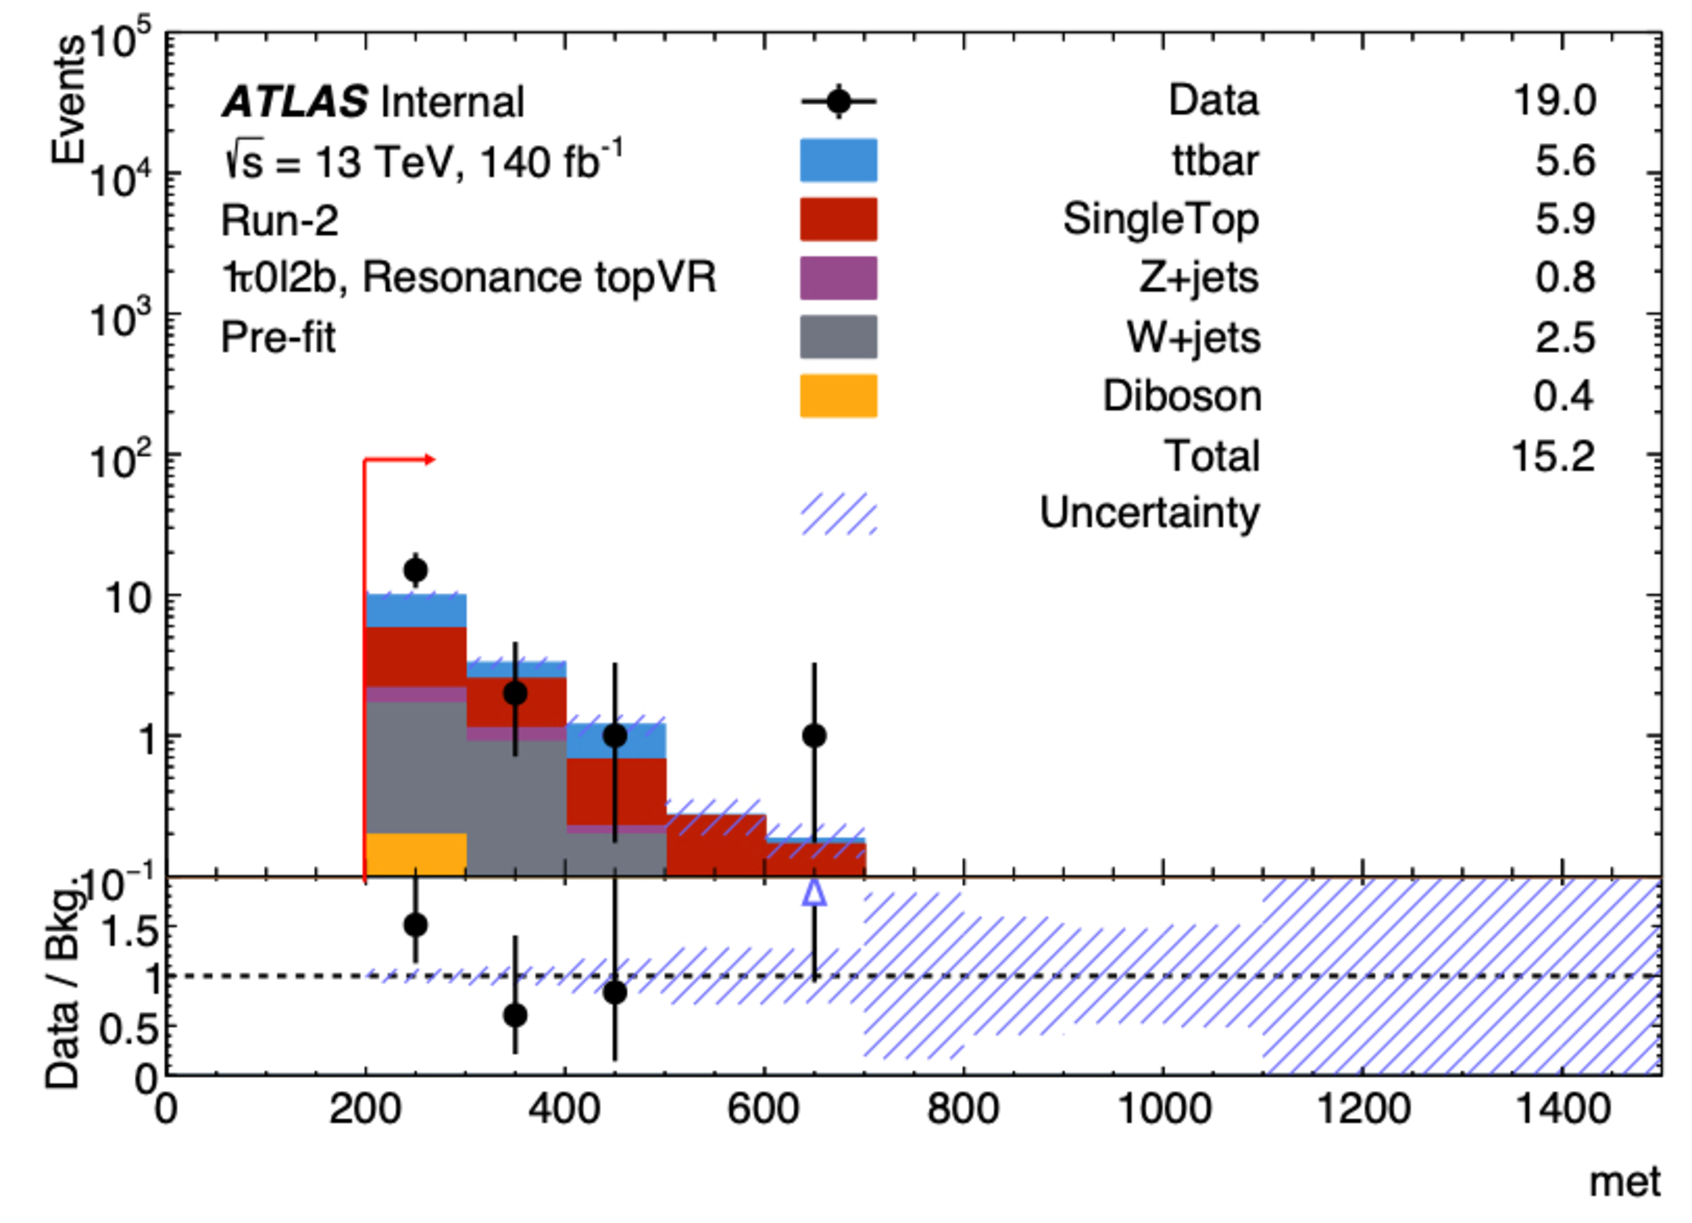
\includegraphics[width=\linewidth]{Figs/CH8/VRTop_Res_met.pdf}
        \caption[]{$\met$}
    \end{subfigure}\hfill
    \begin{subfigure}{0.47\linewidth}
        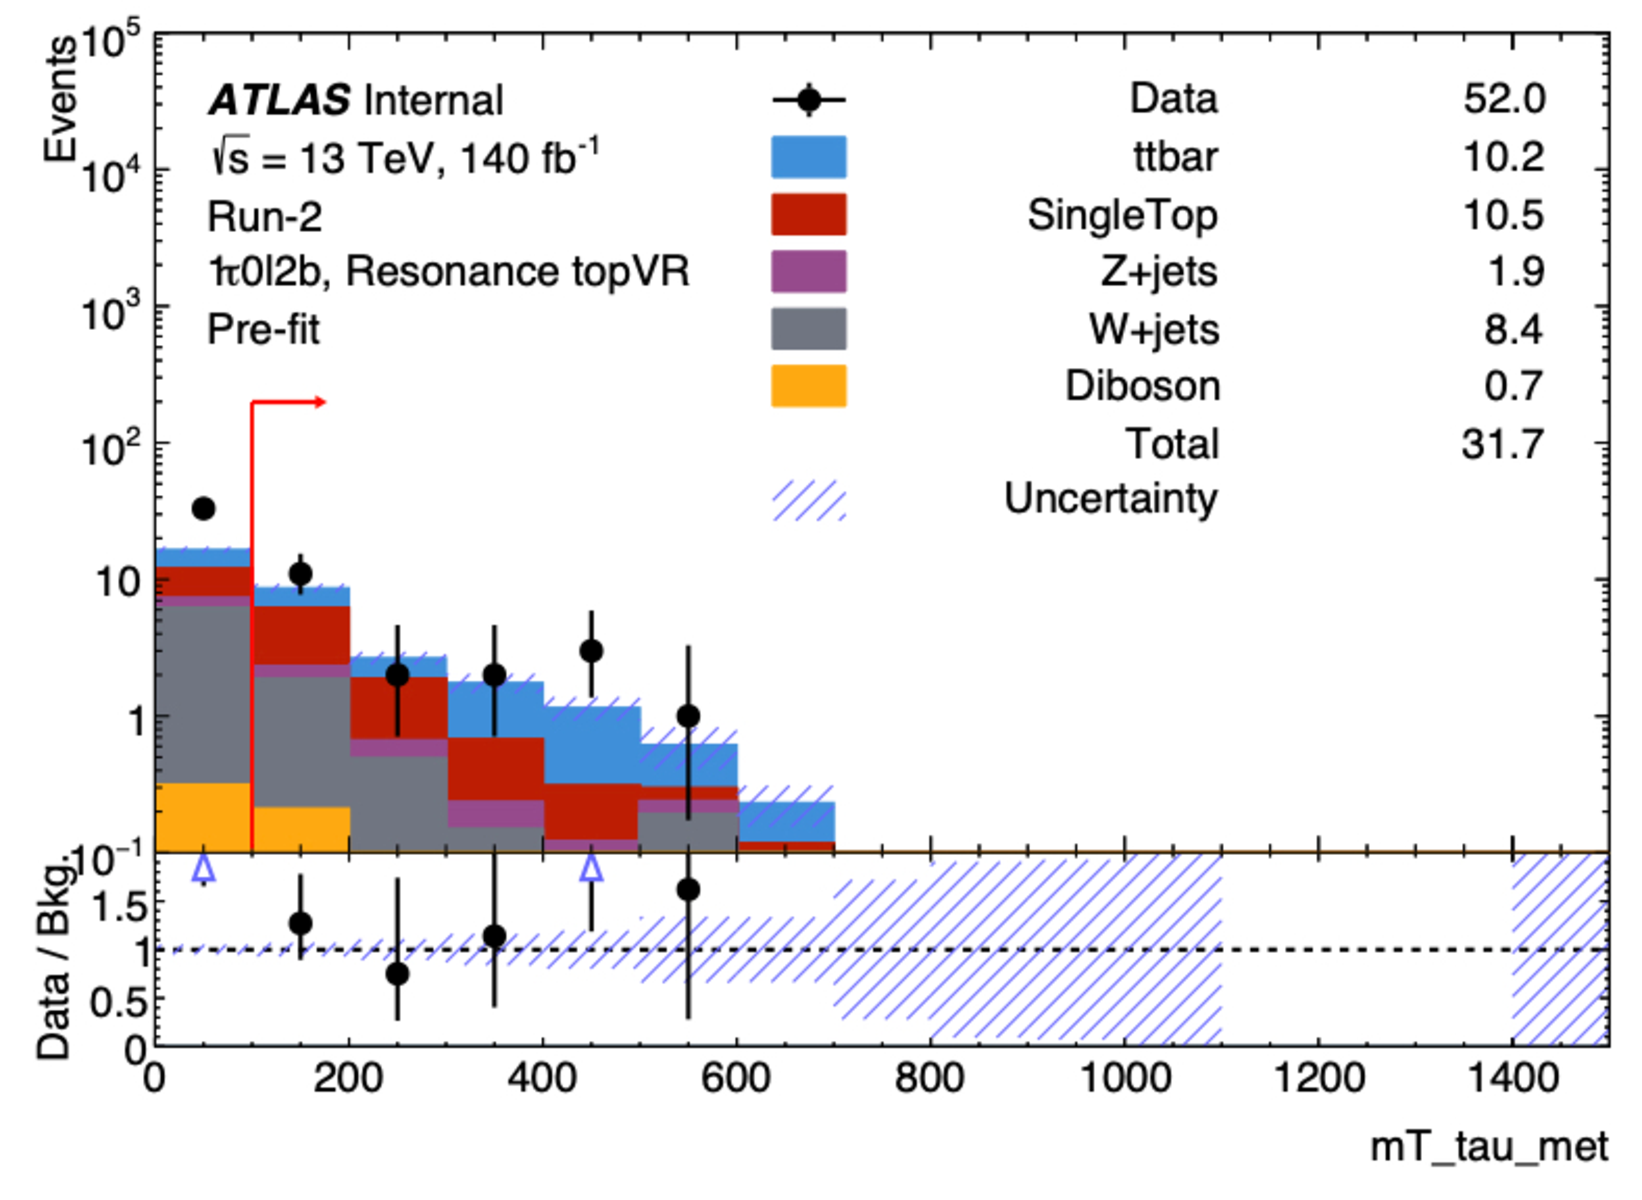
\includegraphics[width=\linewidth]{Figs/CH8/VRTop_Res_mT.pdf}
        \caption[]{$\mT$}
    \end{subfigure}\par\medskip
    \begin{subfigure}{0.47\linewidth}
        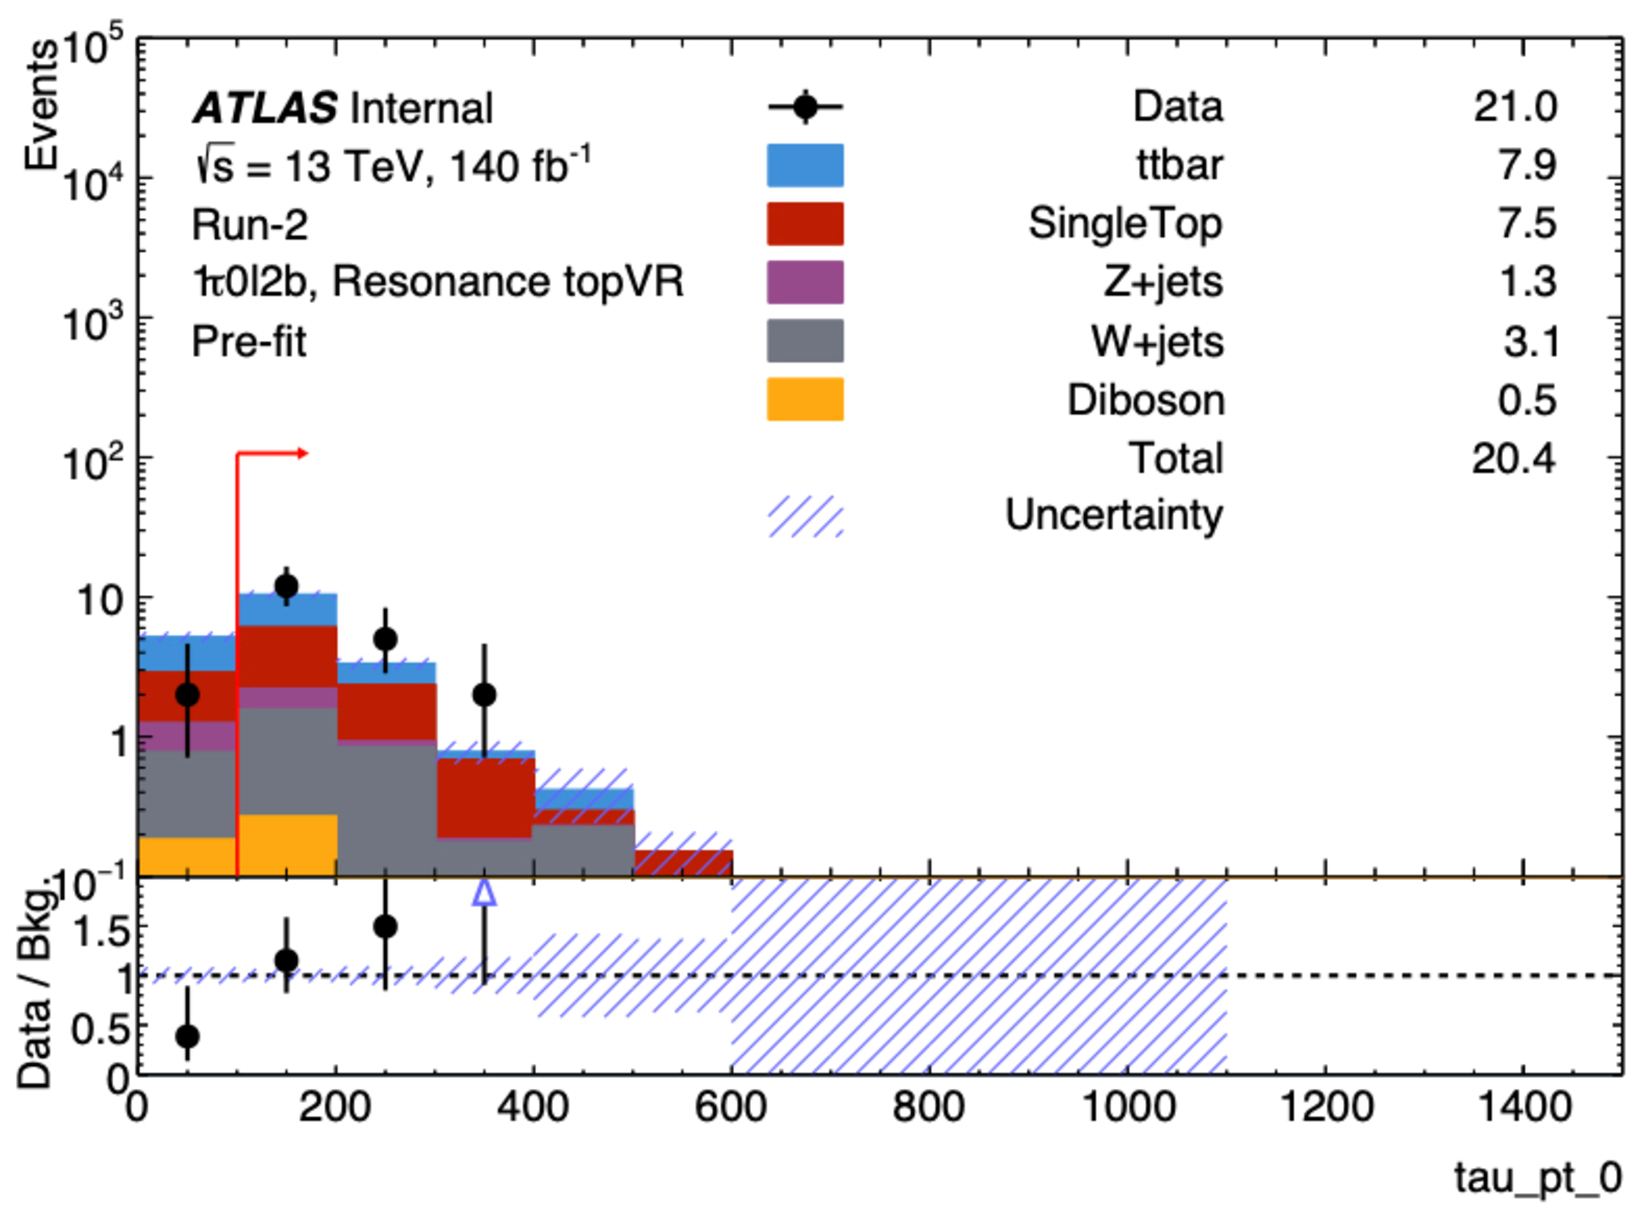
\includegraphics[width=\linewidth]{Figs/CH8/VRTop_Res_tau_pT.pdf}
        \caption[]{$\pT^\tau$}
    \end{subfigure}\hfill
    \begin{subfigure}{0.47\linewidth}
        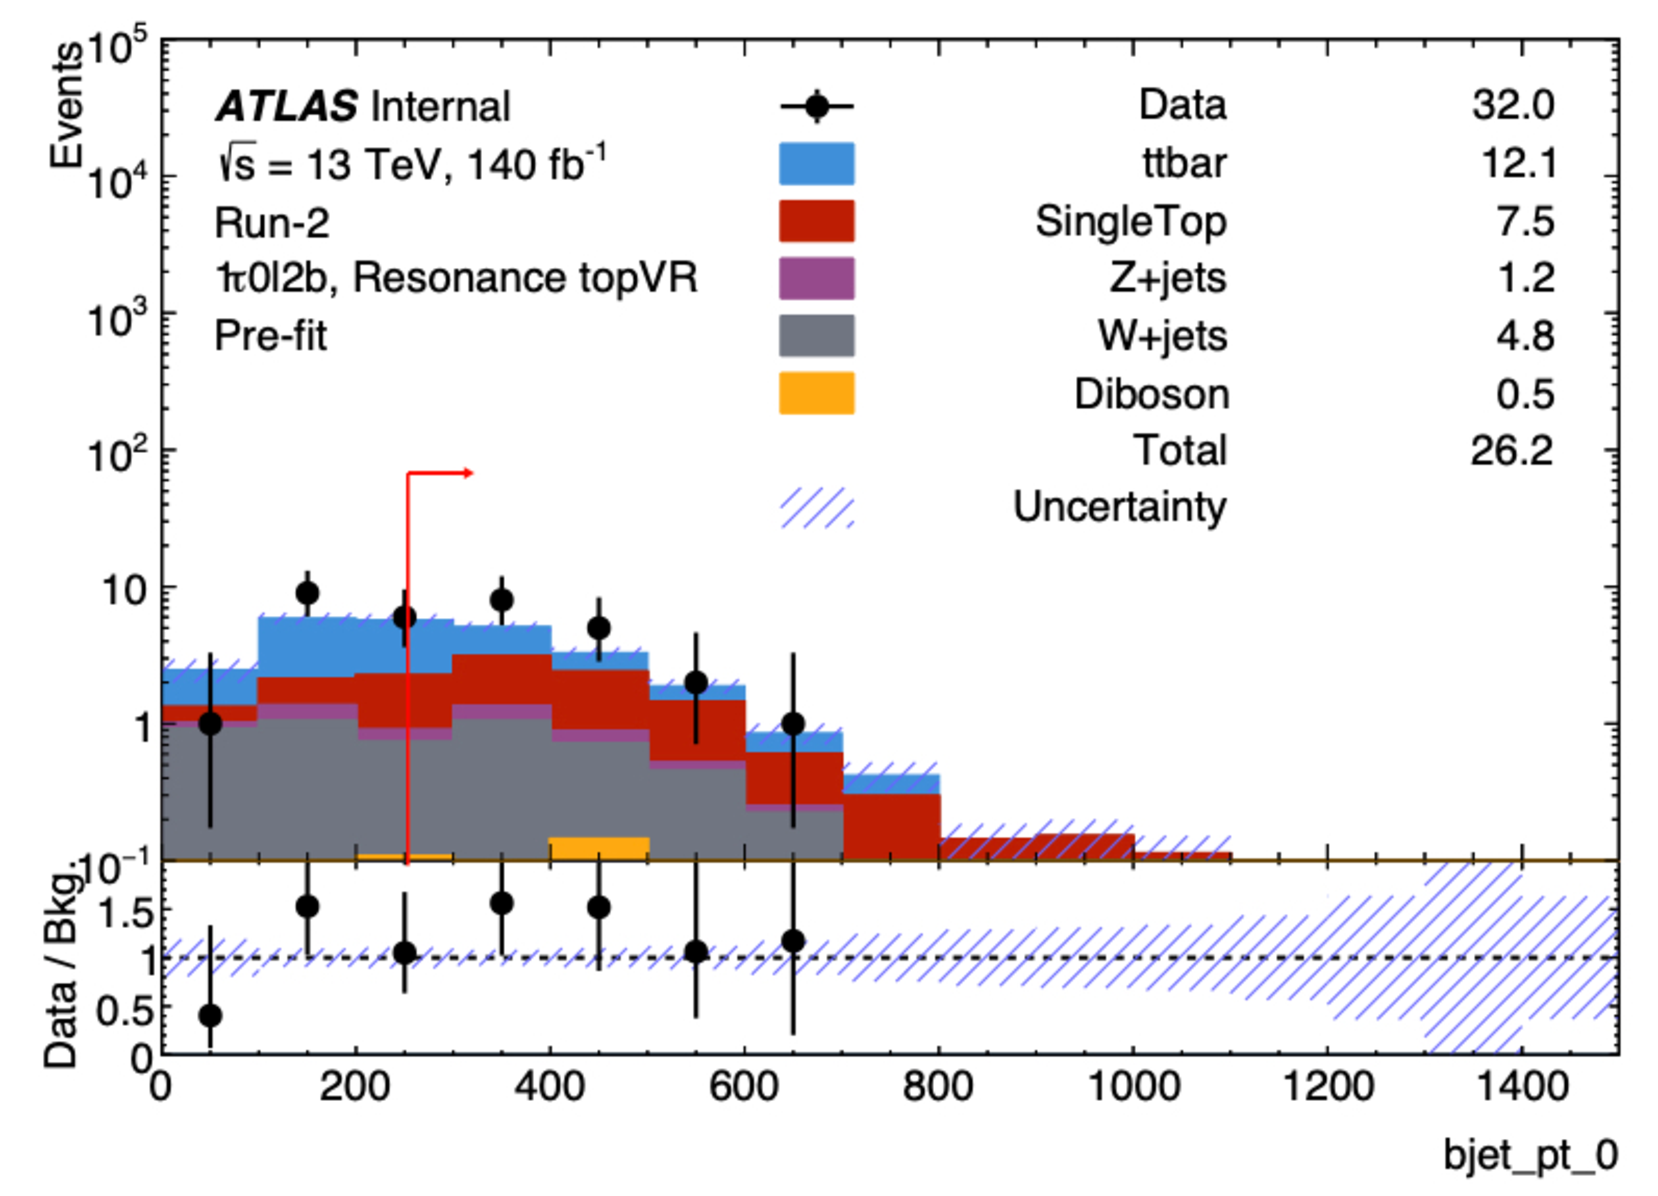
\includegraphics[width=\linewidth]{Figs/CH8/VRTop_Res_bjet_pT.pdf}
        \caption[]{$\pT^b$}
    \end{subfigure}\par\medskip
    \begin{subfigure}{0.47\linewidth}
        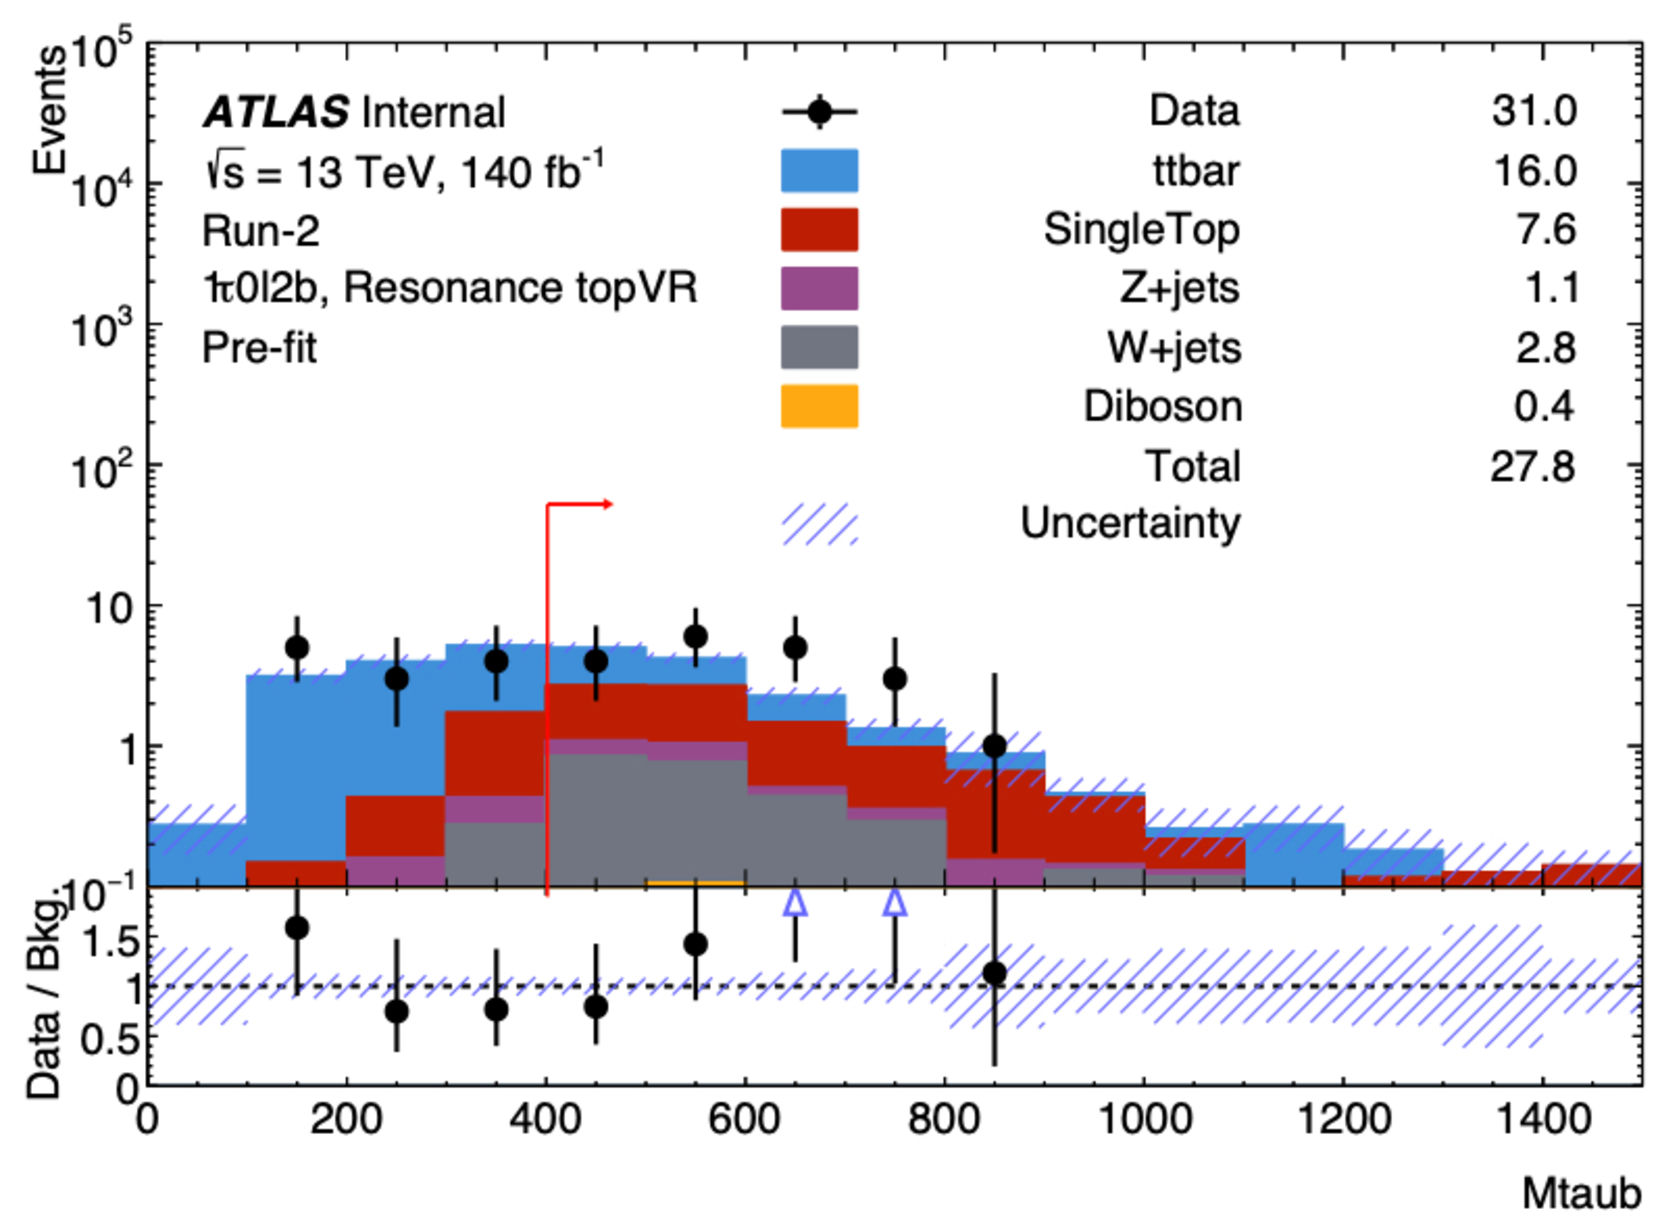
\includegraphics[width=\linewidth]{Figs/CH8/VRTop_Res_InvM.pdf}
        \caption[]{$m_{b\tau}$}
    \end{subfigure}\hfill
    \begin{subfigure}{0.47\linewidth}
        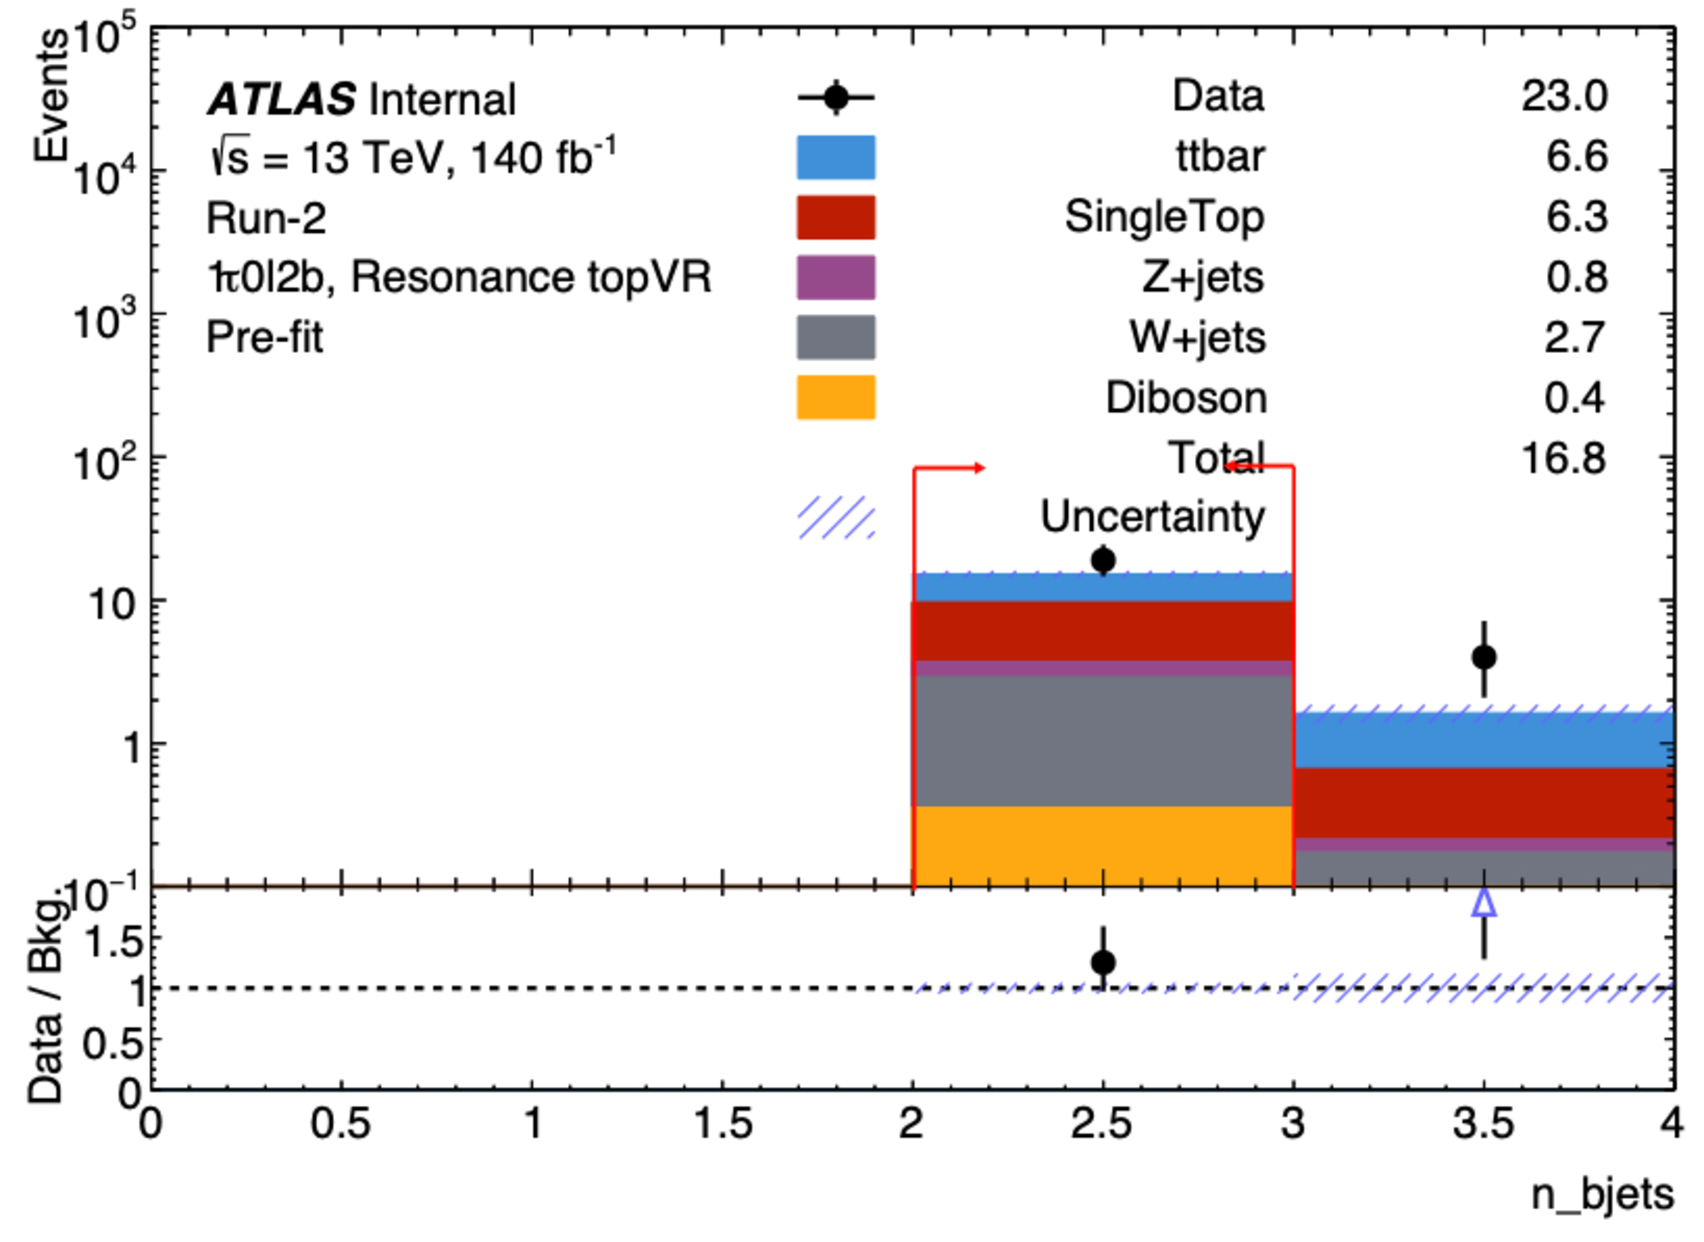
\includegraphics[width=\linewidth]{Figs/CH8/VRTop_Res_nbjets.pdf}
        \caption[]{$N_b$}
    \end{subfigure}\par\medskip
    \caption[Pre-fit N-1 distributions in VRTop-Res]{Pre-fit $N-1$ distributions in VRTop-Res. The lower panels show data divided by the total simulated background. The hatched bands represent the statistical uncertainty in the prediction. The last bin includes the overflow. The leading tagged jet is used for the jet-dependent variables.}
    \label{fig:ch8_vrtop_res}
\end{figure}

\begin{figure}[p]
    \centering
    \begin{subfigure}{0.47\linewidth}
        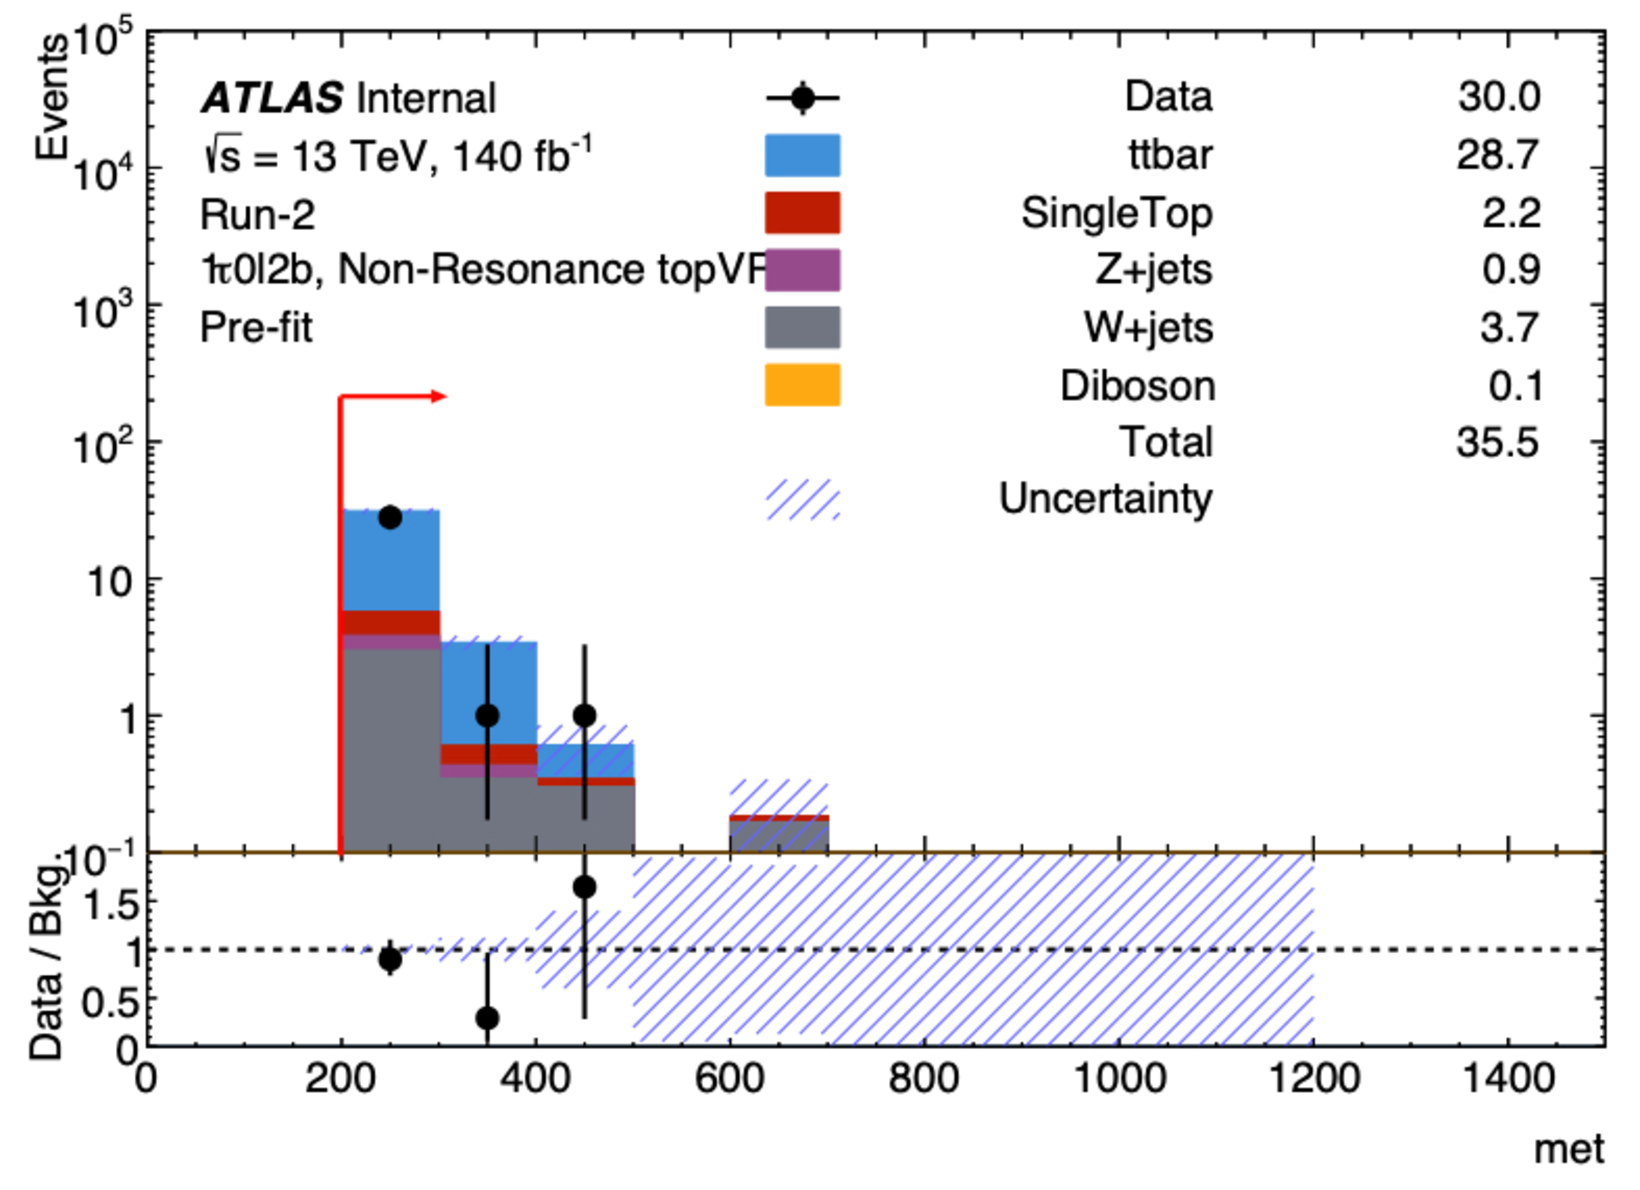
\includegraphics[width=\linewidth]{Figs/CH8/VRTop_NonRes_met.pdf}
        \caption[]{$\met$}
    \end{subfigure}\hfill
    \begin{subfigure}{0.47\linewidth}
        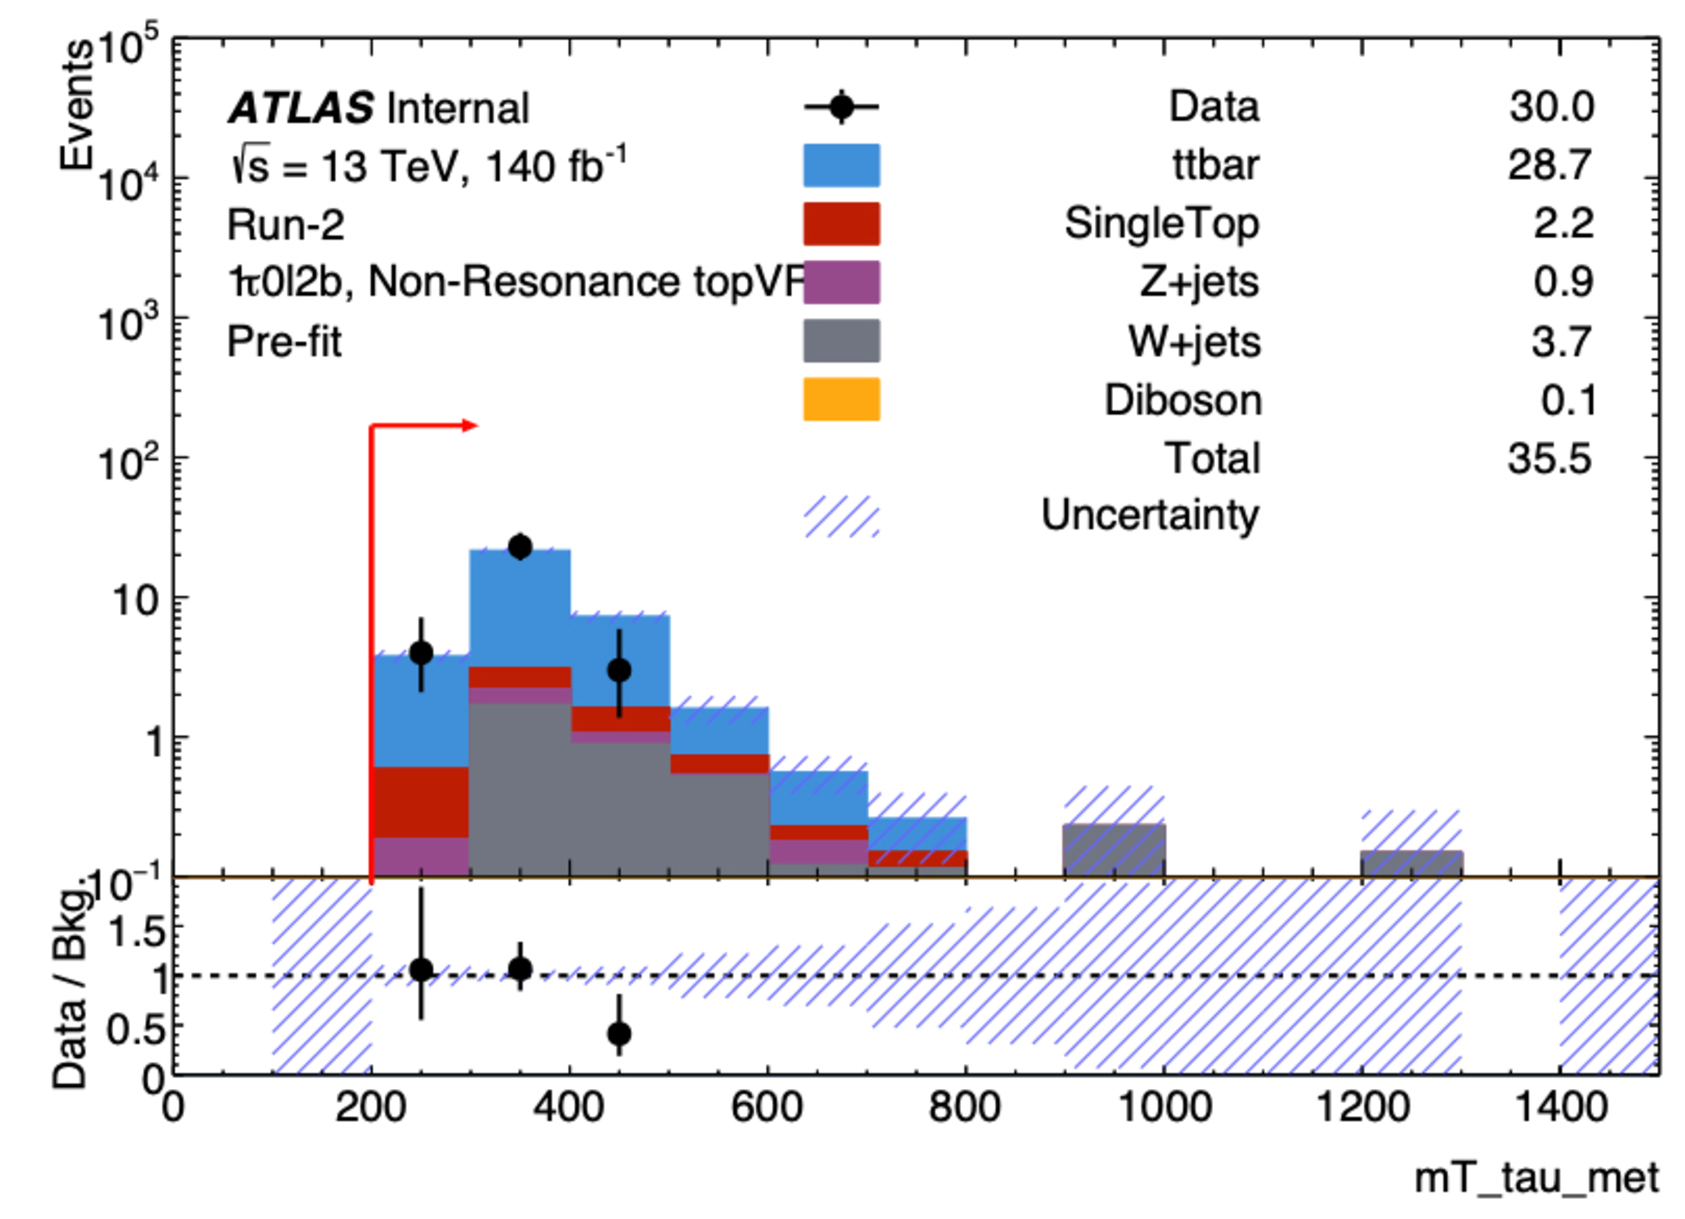
\includegraphics[width=\linewidth]{Figs/CH8/VRTop_NonRes_mT.pdf}
        \caption[]{$\mT$}
    \end{subfigure}\par\medskip
    \begin{subfigure}{0.47\linewidth}
        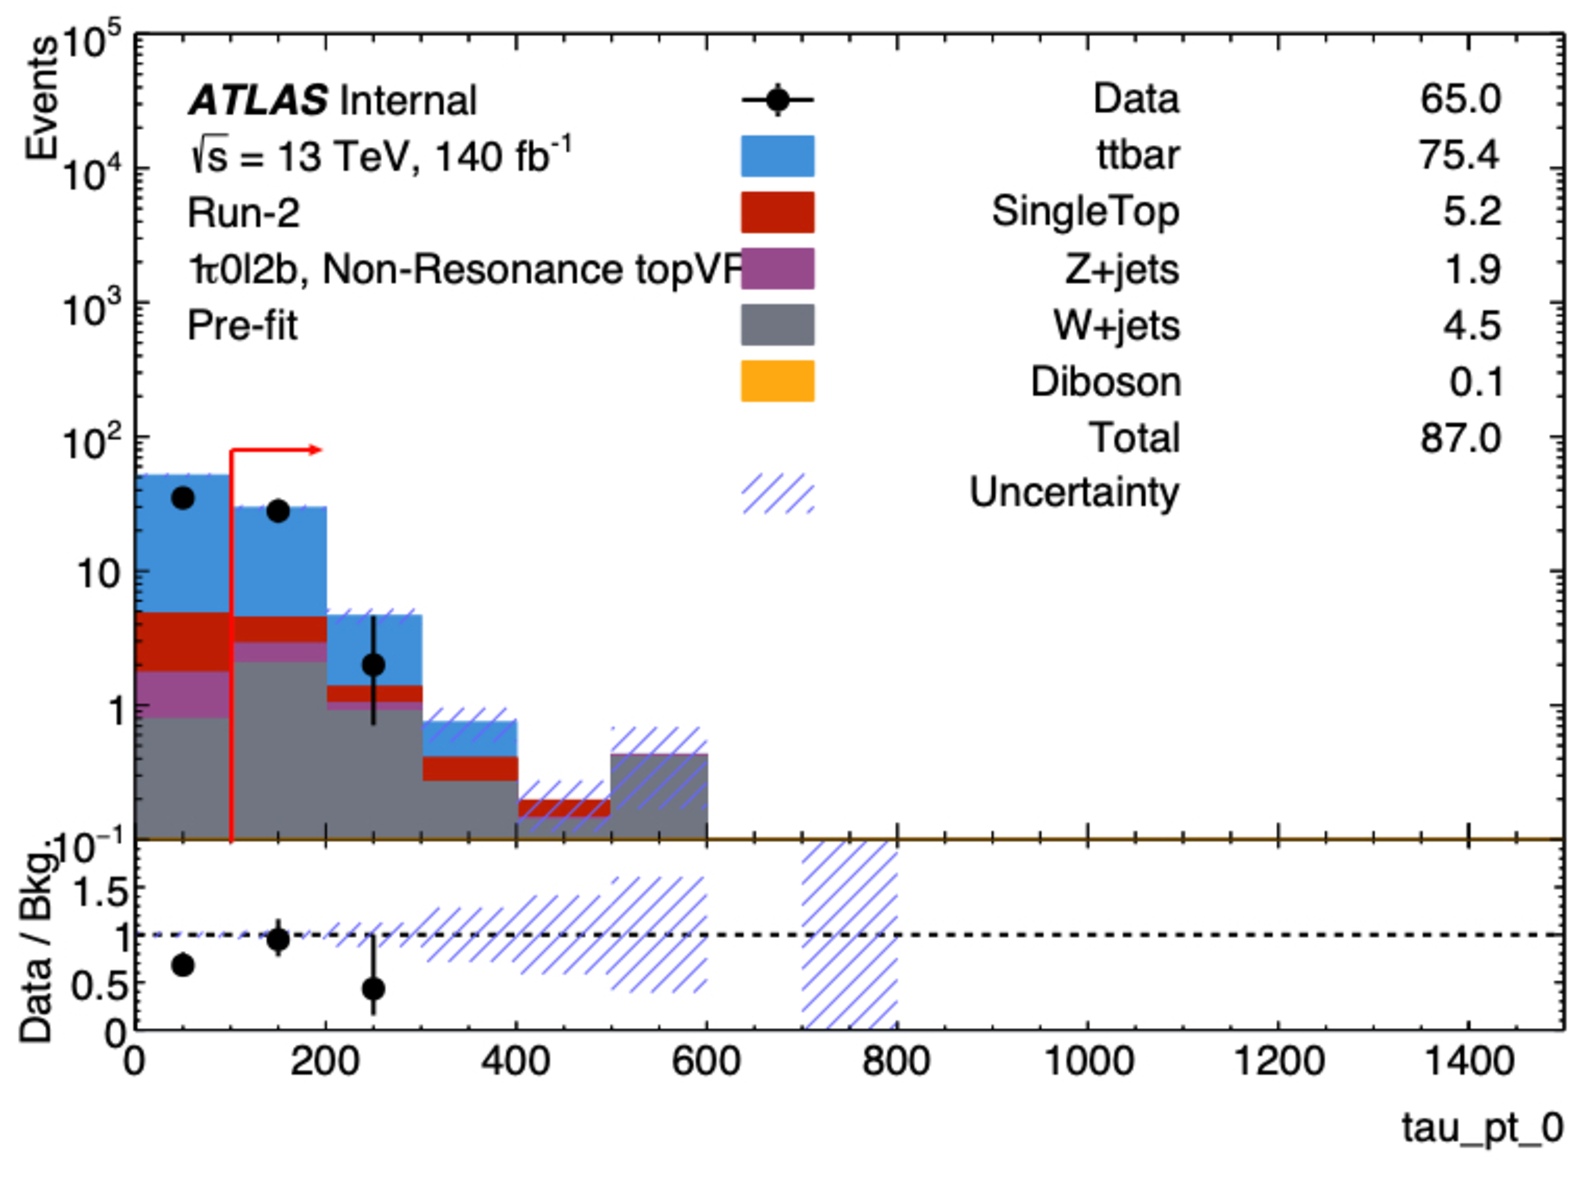
\includegraphics[width=\linewidth]{Figs/CH8/VRTop_NonRes_tau_pT.pdf}
        \caption[]{$\pT^\tau$}
    \end{subfigure}\hfill
    \begin{subfigure}{0.47\linewidth}
        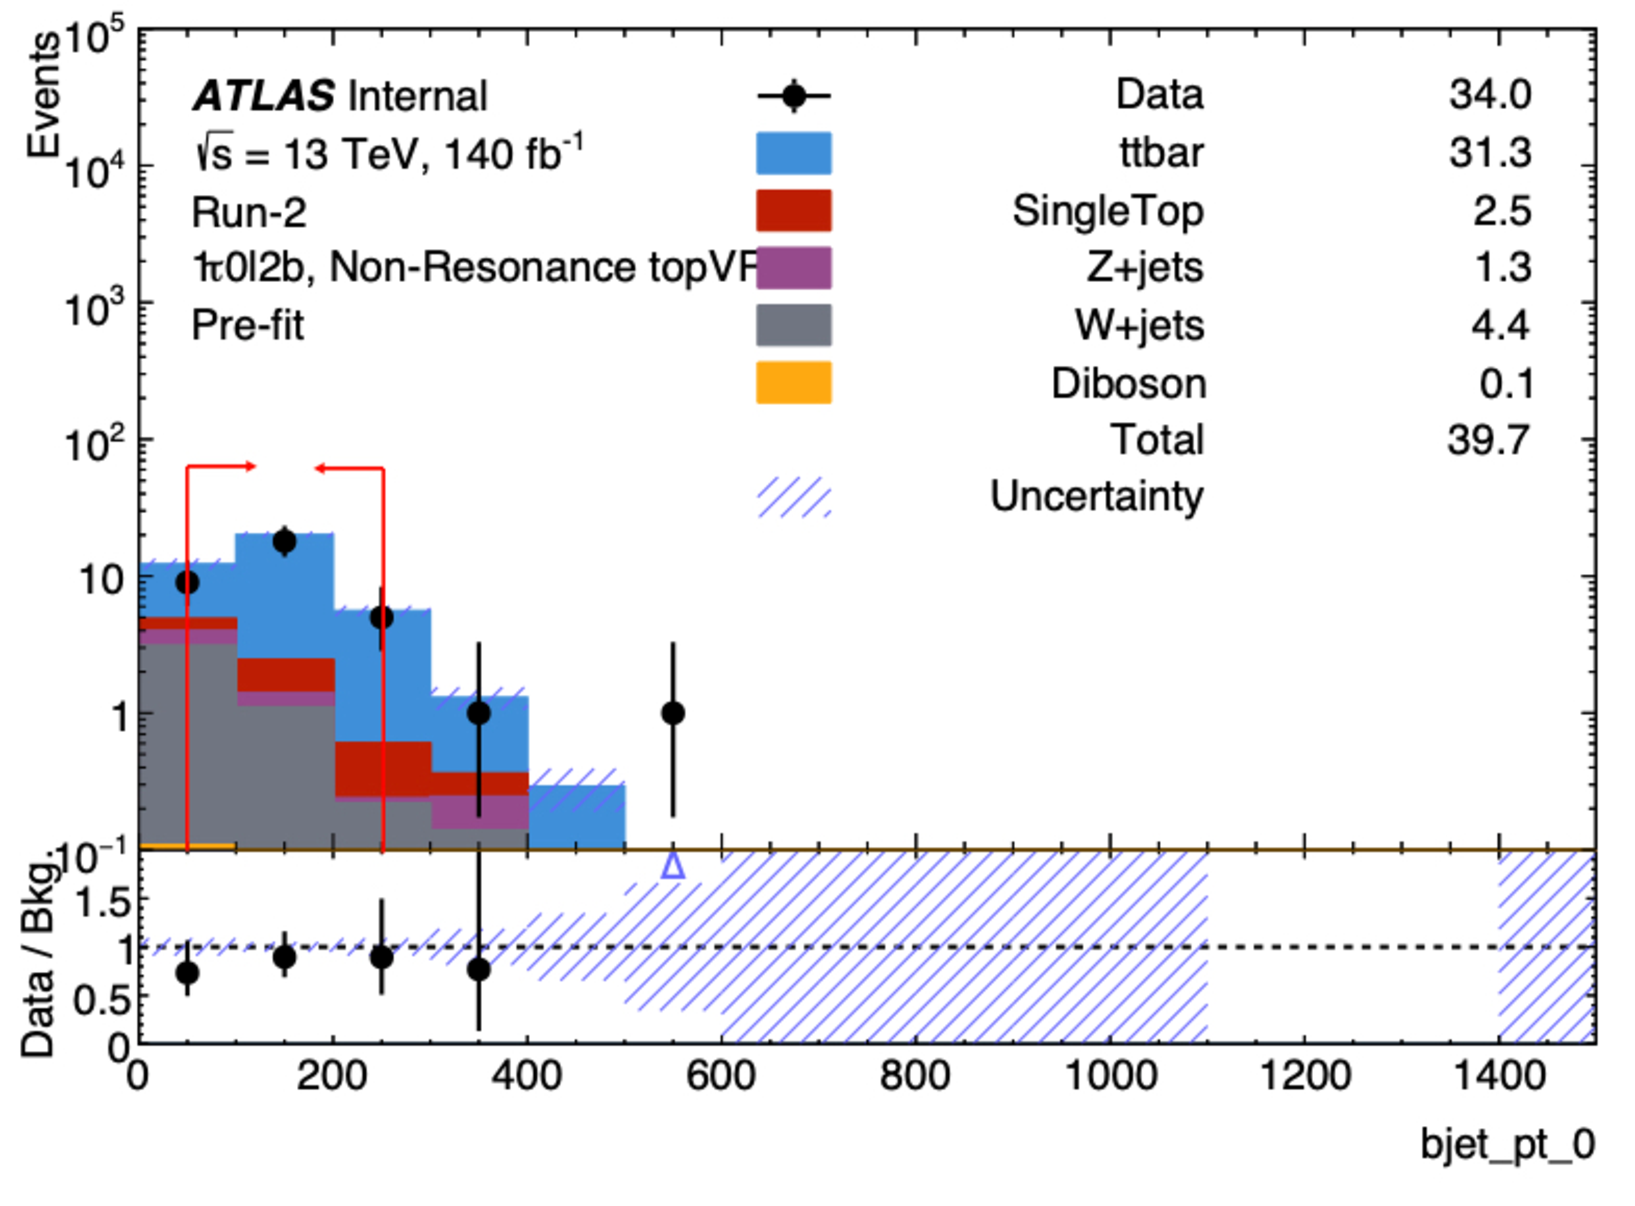
\includegraphics[width=\linewidth]{Figs/CH8/VRTop_NonRes_bjet_pT.pdf}
        \caption[]{$\pT^b$}
    \end{subfigure}\par\medskip
    \begin{subfigure}{0.47\linewidth}
        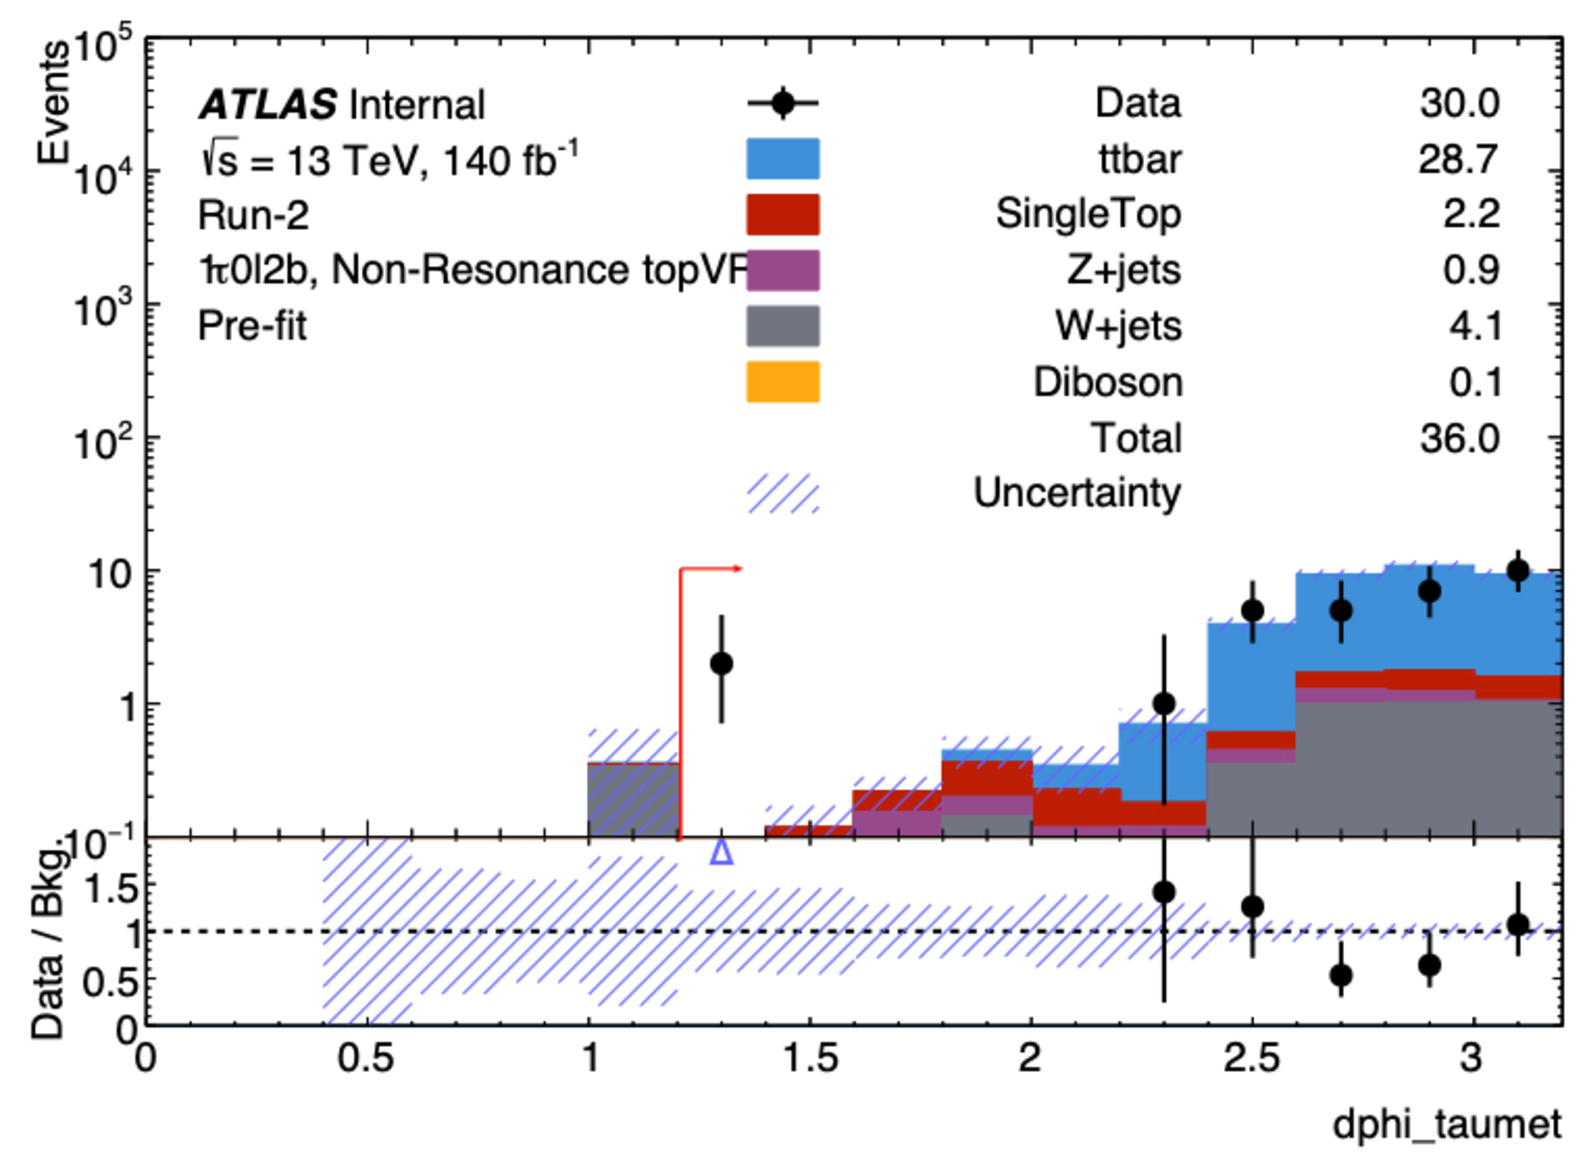
\includegraphics[width=\linewidth]{Figs/CH8/VRTop_NonRes_DPhi.pdf}
        \caption[]{$\DphiTauMet$}
    \end{subfigure}\hfill
    \begin{subfigure}{0.47\linewidth}
        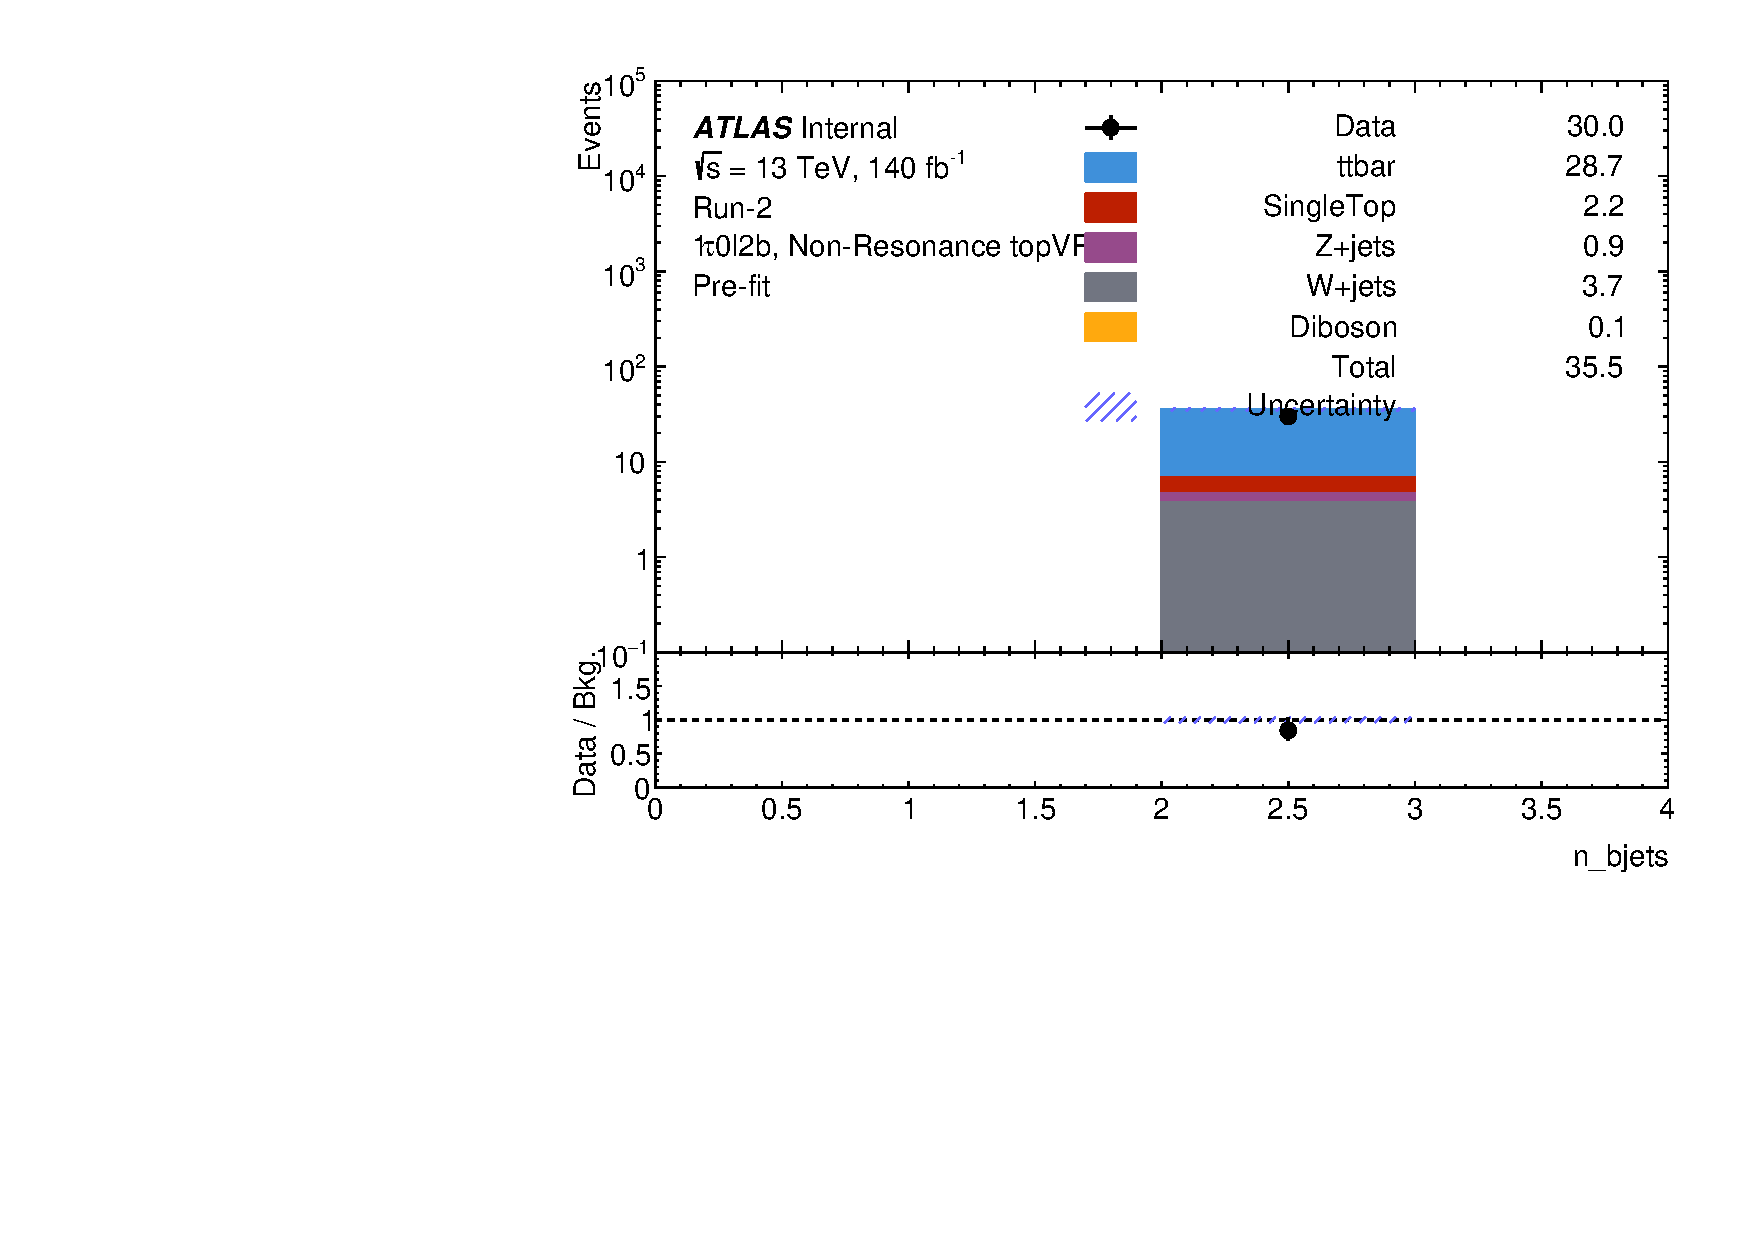
\includegraphics[width=\linewidth]{Figs/CH8/VRTop_NonRes_nbjets.pdf}
        \caption[]{$N_b$}
    \end{subfigure}\par\medskip
    \caption[Pre-fit N-1 distributions in VRTop-NonRes]{Pre-fit $N-1$ distributions in VRTop-NonRes. The lower panels show data divided by the total simulated background. The hatched bands represent the statistical uncertainty in the prediction. The last bin includes the overflow. The leading tagged jet is used for the jet-dependent variables.}
    \label{fig:ch8_vrtop_nonres}
\end{figure}
